% Created 2024-09-02 Mon 14:49
% Intended LaTeX compiler: pdflatex
\documentclass[11pt]{article}
\usepackage[utf8]{inputenc}
\usepackage[T1]{fontenc}
\usepackage{graphicx}
\usepackage{longtable}
\usepackage{wrapfig}
\usepackage{rotating}
\usepackage[normalem]{ulem}
\usepackage{amsmath}
\usepackage{amssymb}
\usepackage{capt-of}
\usepackage{hyperref}
\usepackage{minted}
\usepackage{xcolor}
\usepackage{hyperref}
\usepackage{tocloft}
\usepackage[margin=1.8cm]{geometry}
\usepackage{fancyheadings}
\usepackage{minted}
\usepackage[utf8]{inputenc}
\usepackage{amsmath}
\usepackage{amsfonts}
\usepackage{amssymb}
\usepackage{titlesec}
\usemintedstyle{manni}
\usepackage{enumitem}
\usepackage{pdfpages}
\setlength{\parindent}{0cm}
\usepackage{parskip}
\usemintedstyle{friendly}
\usepackage{graphicx}
\usepackage{listings}
\usepackage{float}
\usepackage{colortbl}
\usepackage{booktabs}
\usepackage{wrapfig}
\usepackage{tabularx}
\usepackage{color}
\usepackage{tabularray}
\restylefloat{table}
\usemintedstyle{dracula}
\usepackage[table]{xcolor}
\usepackage{setspace}
\usepackage[none]{hyphenat}
\usepackage{xcolor}
\usepackage{pagecolor}
\definecolor{solarizedBase03}{RGB}{0, 43, 54}
\definecolor{solarizedBase02}{RGB}{7, 54, 66}
\definecolor{solarizedBase01}{RGB}{88, 110, 117}
\definecolor{solarizedBase00}{RGB}{101, 123, 131}
\definecolor{solarizedBase0}{RGB}{131, 148, 150}
\definecolor{solarizedBase1}{RGB}{147, 161, 161}
\definecolor{solarizedBase2}{RGB}{238, 232, 213}
\definecolor{solarizedBase3}{RGB}{253, 246, 227}
\definecolor{solarizedYellow}{RGB}{181, 137, 0}
\definecolor{solarizedOrange}{RGB}{203, 75, 22}
\definecolor{solarizedRed}{RGB}{220, 50, 47}
\definecolor{solarizedMagenta}{RGB}{211, 54, 130}
\definecolor{solarizedViolet}{RGB}{108, 113, 196}
\definecolor{solarizedBlue}{RGB}{38, 139, 210}
\definecolor{solarizedCyan}{RGB}{42, 161, 152}
\definecolor{solarizedGreen}{RGB}{133, 153, 0}
\pagecolor{solarizedBase3}
\color{solarizedBase00}
\hypersetup{
colorlinks=true,
linkcolor=solarizedBlue,
filecolor=solarizedGreen,
urlcolor=solarizedOrange,
citecolor=solarizedMagenta,
}
\titleformat{\section}
{\color{solarizedBlue}\normalfont\Large\bfseries}
{\color{solarizedBlue}\thesection}{1em}{}
\titleformat{\subsection}
{\color{solarizedGreen}\normalfont\large\bfseries}
{\color{solarizedGreen}\thesubsection}{1em}{}
\titleformat{\subsubsection}
{\color{solarizedYellow}\normalfont\normalsize\bfseries}
{\color{solarizedYellow}\thesubsubsection}{1em}{}
\definecolor{draculaBackground}{HTML}{282a36}
\definecolor{draculaForeground}{HTML}{f8f8f2}
\definecolor{draculaSelection}{HTML}{44475a}
\definecolor{draculaComment}{HTML}{6272a4}
\definecolor{draculaCyan}{HTML}{8be9fd}
\definecolor{draculaGreen}{HTML}{50fa7b}
\definecolor{draculaOrange}{HTML}{ffb86c}
\definecolor{draculaPink}{HTML}{ff79c6}
\definecolor{draculaPurple}{HTML}{bd93f9}
\definecolor{draculaRed}{HTML}{ff5555}
\definecolor{draculaYellow}{HTML}{f1fa8c}
\usepackage[table,xcdraw]{xcolor}
\author{Robert Alicea}
\date{\today}
\title{P.S. 192 Family Handbook 2023-24}
\hypersetup{
 pdfauthor={Robert Alicea},
 pdftitle={P.S. 192 Family Handbook 2023-24},
 pdfkeywords={},
 pdfsubject={},
 pdfcreator={Emacs 29.4 (Org mode 9.6.15)}, 
 pdflang={English}}
\begin{document}


\includepdf[pages=1,fitpaper]{pdf1.pdf}

\pagenumbering{\fancyhf{}}
\pagestyle{headings}
\pagenumbering{arabic}

\fancyhead[R]{\thepage}

\fancyfoot[C]{The School of joyful Learning \& Infinite Potential}
\pagestyle{fancy}
\renewcommand{\footrulewidth}{1px}

\definecolor{dkgreen}{rgb}{0,0.6,0}
\definecolor{gray}{rgb}{0.5,0.5,0.5}
\definecolor{mauve}{rgb}{0.58,0,0.82}

\clearpage
\clearpage \tableofcontents \clearpage

\section{Introduction}
\label{sec:orga154fad}
Welcome to PS192, where every day is an adventure in joyful learning! This book is about two very special characters, Leo and Lea, who learn about the values of justice, honor, and self-discipline through magical experiences at their school. As you read their story, you’ll discover how you can be a bucket filler, just like Leo and Lea, and make PS192 a place where everyone feels safe, respected, and happy.
\begin{figure}[b]  % The 'b' option places the figure at the bottom of the page
  \centering 
\includegraphics[width=.5\textwidth]{/home/rob/ps192_welcome_letters/butket-filler/himher1.png}
  \label{fig:fronpage bottom_image}
\end{figure}

\newpage
\begin{figure}[h]  % The 'b' option places the figure at the bottom of the page
  \centering 
\includegraphics[width=1\textwidth]{/home/rob/ps192_welcome_letters/butket-filler/chapter1.opti.png}
  \label{fig:fronpage bottom_image}
\end{figure}
\subsection{Chapter 1: The Magical School Bell}
\label{sec:org49579b5}
Leo the Lion and Lea the Lioness were excited for their first day at PS192. They had heard that it was a very special school, filled with joy and magic. As they walked through the big doors, they heard a bell ring. But this was no ordinary bell—this was the magical school bell! It shimmered with colors and sparkled like the stars.

Ms. Joy, their teacher, welcomed them with a big smile. "Leo and Lea," she said, "here at PS192, we believe in filling each other's buckets with kindness and respect. Today, you'll start learning how to do just that!"
\newpage
\begin{figure}[h]  % The 'b' option places the figure at the bottom of the page
  \centering 
\includegraphics[width=1\textwidth]{/home/rob/ps192_welcome_letters/butket-filler/chapter2.opti.png}
  \label{fig:fronpage bottom_image}
\end{figure}
\subsection{Chapter 2: The Hallway of Justice}
\label{sec:org77eb89c}
Ms. Joy led the class down the hallway, which was called the Hallway of Justice. The walls were lined with pictures of students standing up for what is right. There was a golden scale that tipped toward fairness, and whenever someone made a just decision, the scale would glow.

"Justice means treating everyone fairly and standing up for what is right," Ms. Joy explained. Leo and Lea noticed a friend being left out of a game and remembered what Ms. Joy said. They invited the friend to join, and the scale glowed brightly. Leo and Lea felt their buckets fill with happiness.
\newpage
\begin{figure}[h]  % The 'b' option places the figure at the bottom of the page
  \centering 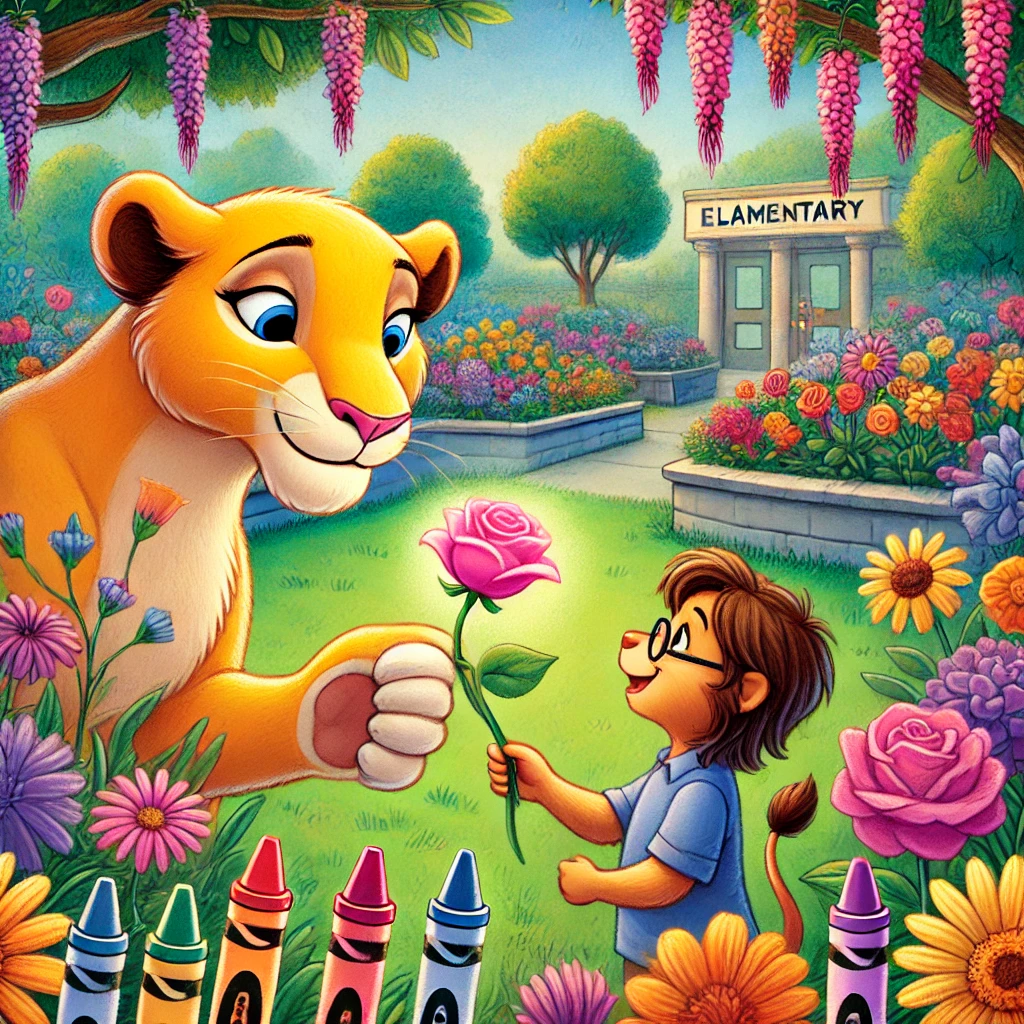
\includegraphics[width=1\textwidth]{/home/rob/ps192_welcome_letters/butket-filler/chapter3.opti.png}
  \label{fig:fronpage bottom_image}
\end{figure}
\subsection{Chapter 3: The Garden of Honor}
\label{sec:orgc990a13}
Next, Ms. Joy took them to the Garden of Honor. The flowers here only bloomed when someone did something honorable. Honor means being truthful, keeping promises, and showing respect.

Leo and Lea saw a flower wilting. "Why is it sad?" Leo asked. Ms. Joy explained that someone had forgotten to return a borrowed book. Lea quickly remembered that she had borrowed a crayon and hadn’t returned it. She ran back to give it to its owner, and the flower bloomed beautifully. Their buckets felt fuller than ever!
\newpage
\begin{figure}[h]  % The 'b' option places the figure at the bottom of the page
  \centering 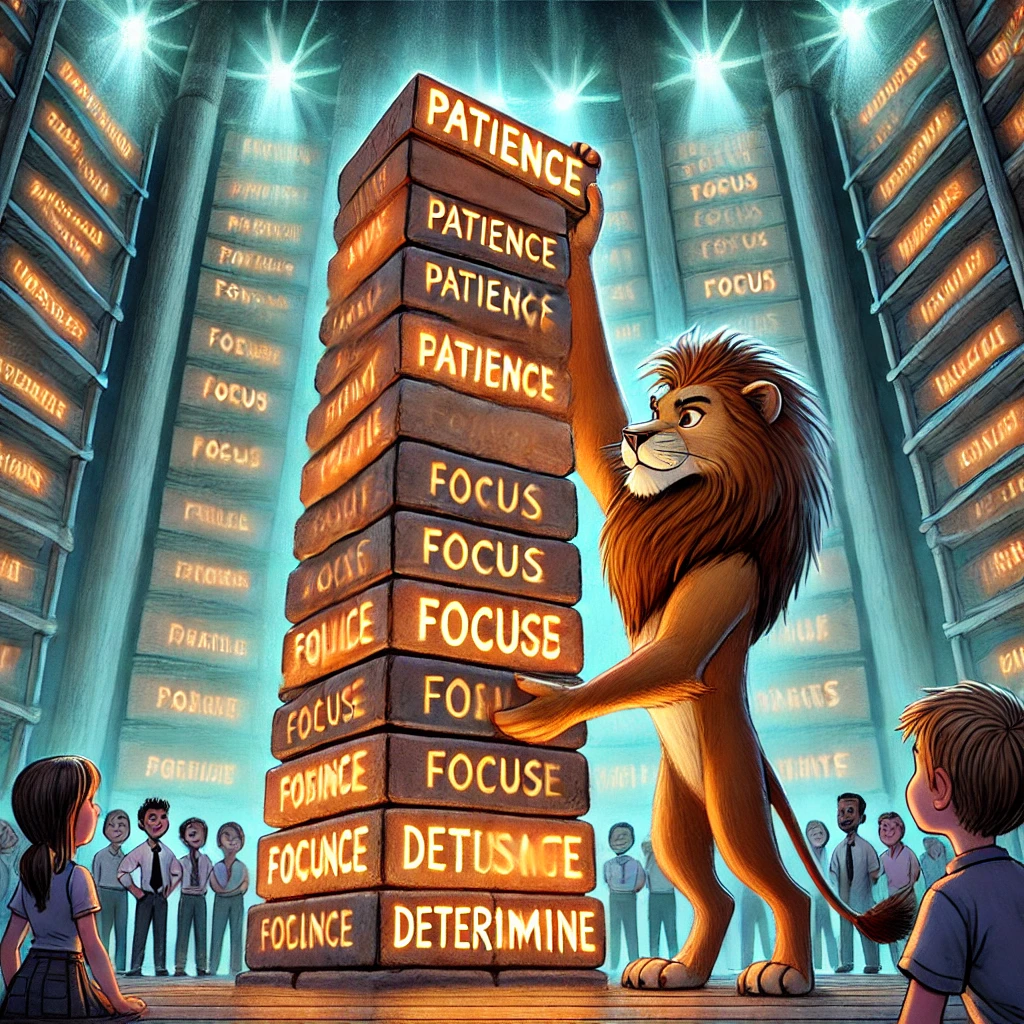
\includegraphics[width=1\textwidth]{/home/rob/ps192_welcome_letters/butket-filler/chapter4.opti.png}
  \label{fig:fronpage bottom_image}
\end{figure}
\subsection{Chapter 4: The Tower of Self-Discipline}
\label{sec:orgea013ee}
Finally, Ms. Joy brought them to the Tower of Self-Discipline. It was tall and strong, built brick by brick by students who practiced self-control and patience. The tower’s bricks were inscribed with words like "Patience," "Focus," and "Determination."

Leo was tempted to run ahead and play, but he remembered the lesson about self-discipline. He took a deep breath, waited his turn, and focused on the task. Another brick appeared on the tower with his name on it, and his bucket filled with pride.
\newpage
\begin{figure}[h]  % The 'b' option places the figure at the bottom of the page
  \centering 
\includegraphics[width=1\textwidth]{/home/rob/ps192_welcome_letters/butket-filler/final-chapter.opti.png}
  \label{fig:fronpage bottom_image}
\end{figure}
\subsection{Chapter 5: The Bucket Filler's Secret}
\label{sec:orgb6a557d}
At the end of the day, Ms. Joy gathered everyone. "You’ve all done something amazing today," she said. "By practicing justice, honor, and self-discipline, you’ve filled your buckets and others’. That’s the secret of being a bucket filler—when you help others feel good, you feel good too!"

Leo and Lea looked at their buckets, now overflowing with happiness. They knew that every day at PS192 would be an opportunity to fill more buckets, make new friends, and grow together.

\newpage
\section{Classroom Material}
\label{sec:org79a1bf5}
\subsection{Activity 1: Create Your Own Bucket}
\label{sec:org4b59c96}
\begin{itemize}
\item \textbf{\textbf{Objective:}} Students will create their own paper bucket to symbolize their goal of being a bucket filler.
\item \textbf{\textbf{Materials:}} Construction paper, crayons, scissors, glue.
\item \textbf{\textbf{Instructions:}} Have students decorate a paper bucket with their name on it. They can add drawings that represent justice, honor, and self-discipline.
\item \textbf{\textbf{Discussion:}} Talk about ways to fill their bucket and others' throughout the school day.
\end{itemize}

\subsection{Activity 2: Justice, Honor, and Self-Discipline Charades}
\label{sec:orgb56ca4d}
\begin{itemize}
\item \textbf{\textbf{Objective:}} Reinforce understanding of the school values through role-play.
\item \textbf{\textbf{Materials:}} None.
\item \textbf{\textbf{Instructions:}} In small groups, students act out scenarios that demonstrate justice, honor, or self-discipline while the others guess the value being displayed.
\item \textbf{\textbf{Discussion:}} Reflect on how these values make the school a better place.
\end{itemize}

\subsection{Activity 3: The Garden of Honor Collage}
\label{sec:orgc5bcc3a}
\begin{itemize}
\item \textbf{\textbf{Objective:}} Encourage students to recognize honorable behavior.
\item \textbf{\textbf{Materials:}} Magazines, glue, large poster board.
\item \textbf{\textbf{Instructions:}} Have students cut out pictures that represent honor (e.g., helping others, sharing) and create a class collage.
\item \textbf{\textbf{Discussion:}} Display the collage as a reminder to practice honor daily.
\end{itemize}

\subsection{Activity 4: The Tower of Self-Discipline Building Challenge}
\label{sec:orged7bd11}
\begin{itemize}
\item \textbf{\textbf{Objective:}} Practice self-discipline in a group setting.
\item \textbf{\textbf{Materials:}} Blocks or stacking toys.
\item \textbf{\textbf{Instructions:}} Students work together to build the tallest tower they can, but they must do it slowly and carefully, practicing patience and teamwork.
\item \textbf{\textbf{Discussion:}} Discuss how self-discipline helped them achieve their goal.
\end{itemize}
\newpage
\section{Teacher Plan}
\label{sec:orgdaaa5f3}
\subsection{Day 1: Introduction to Bucket Filling}
\label{sec:org844715f}
\begin{itemize}
\item Read "Leo and Lea's Magical Adventure at PS192." Discuss the concept of bucket filling.
\item Activity: Create Your Own Bucket.
\item Discuss and role-play (Activity 2) the values of justice, honor, and self-discipline.
\end{itemize}

\subsection{Day 2: Deep Dive into Values}
\label{sec:org73404ac}
\begin{itemize}
\item Focus on Justice. Revisit the Hallway of Justice from the story. Discuss examples.
\item Activity: The Garden of Honor Collage.
\item Focus on Honor. Discuss how keeping promises and telling the truth are ways to fill buckets.
\end{itemize}

\subsection{Day 3: Building Self-Discipline}
\label{sec:org731e2f6}
\begin{itemize}
\item Focus on Self-Discipline. Revisit the Tower of Self-Discipline from the story.
\item Activity: The Tower of Self-Discipline Building Challenge.
\item Reflection circle. Have students share how they’ve filled a bucket this week.
\end{itemize}

\subsection{Day 4: Practice and Reflection}
\label{sec:orgf182080}
\begin{itemize}
\item Review all the values. How can we be bucket fillers every day?
\item Re-read "Leo and Lea's Magical Adventure at PS192." Have students draw their favorite part and explain why.
\item Class discussion and bucket-filling celebration. Hand out "Bucket Filler of the Month" certificates to students who have consistently practiced the values.
\end{itemize}
\newpage
\section{Additional Tools for Teachers}
\label{sec:org0957dfd}
\subsection{Bucket Filler Chart}
\label{sec:orgd885733}
\begin{itemize}
\item \textbf{\textbf{Purpose:}} Track acts of bucket filling in the classroom.
\item \textbf{\textbf{How to Use:}} Each time a student fills a bucket (justice, honor, or self-discipline), place a star or sticker next to their name on the chart.
\end{itemize}

\subsection{Bucket Filler Certificates}
\label{sec:org257a511}
\begin{itemize}
\item \textbf{\textbf{Purpose:}} Acknowledge students who consistently fill others’ buckets.
\item \textbf{\textbf{How to Use:}} At the end of the month, award a certificate to the student(s) who best exemplify the school’s values.
\end{itemize}

\subsection{Reflection Journals}
\label{sec:org076fc7f}
\begin{itemize}
\item \textbf{\textbf{Purpose:}} Encourage students to reflect on how they have filled buckets each day.
\item \textbf{\textbf{How to Use:}} Provide a small journal for each student where they can draw or write about their bucket-filling experiences.
\end{itemize}
\end{document}
